% Created 2025-04-20 Sun 15:59
% Intended LaTeX compiler: pdflatex
\documentclass[11pt]{article}
\usepackage[utf8]{inputenc}
\usepackage[T1]{fontenc}
\usepackage{graphicx}
\usepackage{longtable}
\usepackage{wrapfig}
\usepackage{rotating}
\usepackage[normalem]{ulem}
\usepackage{amsmath}
\usepackage{amssymb}
\usepackage{capt-of}
\usepackage{hyperref}
\author{Laurent Garnier}
\date{\today}
\title{Comment les mathématiques permettent-elles de mesurer et comprendre les inégalités de richesses ?}
\hypersetup{
 pdfauthor={Laurent Garnier},
 pdftitle={Comment les mathématiques permettent-elles de mesurer et comprendre les inégalités de richesses ?},
 pdfkeywords={},
 pdfsubject={},
 pdfcreator={Emacs 29.4 (Org mode 9.6.15)}, 
 pdflang={English}}
\begin{document}

\maketitle
\tableofcontents


\section{Introduction}
\label{sec:org119e086}
\subsection{Accroche}
\label{sec:org65e244a}

En 2024, les 1\% les plus riches de la planète détenaient près de
43\% des richesses mondiales (rapport \href{https://www.oxfamfrance.org/rapports/multinationales-et-inegalites-multiples/}{Oxfam}). Mais comment
mesure-t-on ces inégalités, et que nous disent les mathématiques
sur leurs causes et leurs conséquences ?

\subsection{Problématique}
\label{sec:org0016ef8}

Comment les outils mathématiques (statistiques, indicateurs,
modèles) permettent-ils de quantifier et d’analyser les inégalités
économiques ?

\subsection{Annonce du plan}
\label{sec:orge5e64ce}

\begin{enumerate}
\item \textbf{Mesurer les inégalités} : les indicateurs mathématiques.
\item \textbf{Modéliser les mécanismes} : lois et théories économiques.
\item \textbf{Limites et enjeux} : que ne peuvent pas expliquer les maths ?
\end{enumerate}

\section{Partie 1 : Mesurer les inégalités}
\label{sec:orgb35bae1}
\subsection{Outils statistiques}
\label{sec:orgca35b99}

\begin{itemize}
\item \href{https://fr.wikipedia.org/wiki/Courbe\_de\_Lorenz}{Courbe de Lorenz} : représentation graphique de la répartition des
richesses.

\begin{center}
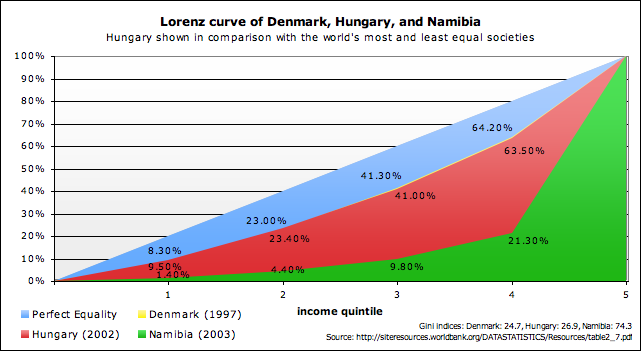
\includegraphics[width=5cm,height=3cm]{./lorenz-curve.png}
\end{center}

\begin{center}
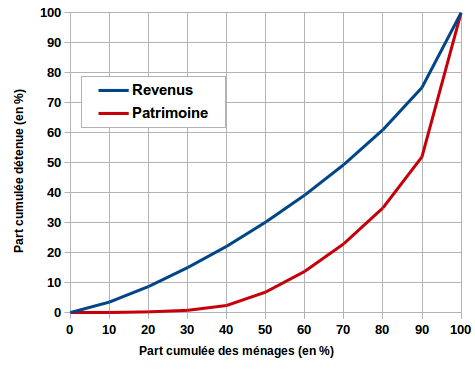
\includegraphics[width=5cm,height=3cm]{./lorenz-france-2010.png}
\end{center}
\end{itemize}
\end{document}
